\chapter{Технологическая часть}

\section{Требования к программе}

К программе предъявляются следующие требования:

\begin{itemize}
	\item программа должна предоставлять пользователю возможность взаимодействовать со слаймом;
	\item оконный интерфейс программы должен предоставлять пользователю возможность изменять такие параметры слайма, как цвет, коэффициент пропускания и показатель поглощения;
	\item должна быть возможность перезагрузки сцены;
\end{itemize}

\section{Выбор инструментов разработки}

Для выполнения данной работы был выбран высокоуровневый язык
программирования C++. Данный выбор обусловлен следующими факторами:

\begin{itemize}
	\item C++ поддерживает технологию объектно-ориентированного
	программирования, которая позволяет легко модифицировать программу и
	эффективно организовывать взаимодействия между объектами;
	\item С++ обладает очень высокими показателями вычислительной
	производительности, что также обеспечивает достойную скорость исполнения
	кода;
	\item для C++ было создано множество библиотек, которые могут быть
	использованы, в частности, для математических расчетов.
\end{itemize}

В качестве среды разработки была выбрана Visual Studio Code по
следующим причинам:

\begin{itemize}
	\item данная среда разработки бесплатна;
	\item в данной среде присутствуют встроенный отладчик, инструменты для
	работы с Git и средства навигации по коду, автодополнения кода и контекстной
	подсказки;
	\item имеется возможность расширить любой функционал, включая
	компиляцию и отладку.
\end{itemize}

\section{Диаграмма классов}

\section{Интерфейс программы}

На рисунке \ref{ui} показан интерфейс программы.

\begin{figure}[H]
	\centering
	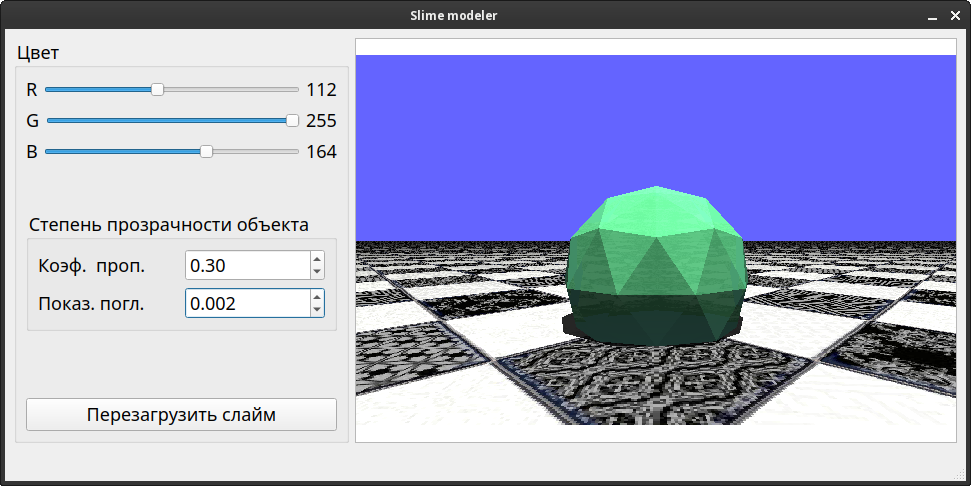
\includegraphics[width=\linewidth]{ui}
	\caption{Интерфейс программы}
	\label{ui}
\end{figure}

\clearpage
